\setchapterstyle{kao}
\setchapterpreamble[u]{\margintoc}
\chapter{Proof-by-Action}
\labch{pba}

% \begin{kaobox}[frametitle=Note]
%   Most of the content in this chapter has been previously published in
%   \cite{10.1145/3497775.3503692}.
% \end{kaobox}

% \section{What is a sequent?}

% In its original formulation by Gentzen\todo{citation of original paper
% introducing the sequent calculus}, a sequent is simply an expression of the form
% $Γ ⊢ C$, where $\Gamma$ is a list of formulas in the logic of interest, and $C$
% is a distinguished formula. In the context of theorem proving, sequents are
% usually seen as \emph{goals}, a denomination dating back to the LCF prover
% \cite{doi:10.1098/rsta.1984.0067}. That is, the statement $C$ corresponds to the
% \emph{conclusion} the user wants to reach that still needs justification, and
% the latter can be achieved by using either \emph{hypotheses} in $\Gamma$, or
% already proved lemmas stored in a global environment\sidenote{From a purely
% proof-theoretical point of view, having a separate global environment is
% unnecessary, and every statement considered justified --- either proved or
% assumed --- can be put in the hypotheses $Γ$.}.

% One can find a number of extensions and variants to the syntax of sequents,
% depending on the logic under consideration. For example, it is customary in
% propositional and predicate logic to describe $Γ$ as a set or multiset, because
% the way hypotheses are ordered is immaterial with regard to provability.

% However many modern proof assistants are based on \emph{dependent type theory},
% where hypotheses have explicit \emph{names} identifying them, corresponding to
% \emph{variables}. Then sequents have the form $x_1 : A_1, …, x_n : A_n ⊢ C$, and
% oftentimes the type $A_i$ of some hypothesis will refer to variables in $x_1, …,
% x_n$, thus creating dependencies between hypotheses. In this case, one wants to
% avoid dependency cycles by forcing $A_i$ to refer only to previously occuring
% variables $x_j$ where $j < i$, hence the order of hypotheses becomes logically
% meaningful. From a usability point of view, it can also be beneficial to let the
% user reorganize hypotheses in the order she deems most readable in the course of
% a proof.

% Another common feature consists in extending $Γ$ with \emph{definitions} of the
% form $x := b : A$, where $b$ is some term \emph{provably} of type
% $A$\sidenote{This type-theoretical encoding of definitions dates back to the
% work of N. G. De Bruijn on Automath, according to \cite{geuvers_proof_2009}.}.
% Then $x$ acts as a name for the body $b$ of the definition, and is not just
% assumed to be of type $A$. The more neutral word \emph{context} is usually
% preferred over the word \emph{hypotheses} to denote this mixed list of
% assumptions and definitions. It is also common to qualify the definitions in
% $\Gamma$, or even the full context $\Gamma$, as being \emph{local}, to
% distinguish them from the \emph{global} environment of lemmas and definitions
% mentioned earlier.

% We mention one last possible variation, which is to replace the conclusion $C$
% by a list of conclusions $Δ$, which ought to be understood \emph{disjunctively}.
% That is, a sequent $Γ ⊢ Δ$ seen as a goal can be read ``at least one of the
% conclusions in Δ must be proved under the context $Γ$''. Although introduced
% originally by Gentzen in the context of classical logic, this syntax can also be
% used for \kl{intuitionistic} logics, for example to implement efficient proof search
% procedures \cite{dyckhoff_contraction-free_1992}. In practice however, we do not
% know of any existing proof assistant using multi-conclusion goals at the user
% interface level.


In this chapter, we focus on how both \emph{click} and \emph{drag-and-drop}
(DnD) actions upon the formulas of a sequent can implement proof construction
operations corresponding to the core logic; that is how they deal with logical
connectives, quantifiers and equality. We present these core principles through
various illustrations and examples in \kl{first-order logic}. The technical and
proof-theoretical foundations for the semantics of DnD actions
% , which constitute the main innovation of this work,
will be investigated more thoroughly in \refch{sfl}.
% , although the most important meta-theoretical
% properties will be exposed here with outlines of their proofs.
More advanced features of the Proof-by-Action paradigm that go beyond the core
logic are illustrated in \refch{advanced}, and \refch{plugin} explains how it
can be integrated in a mainstream proof assistant.

We have started to implement the paradigm in a prototype named {\em Actema} (for
Active Mathematics) running through a web HTML5/JavaScript interface. At the
time of writing, a standalone version of the prototype (i.e. which does not use
an existing theorem prover as its backend) is publicly available online
\cite{Actema:link}\marginnote[240pt]{\textbf{TODO:} Have a more durable way to
access the prototype? More generally, what is the correct way to incorporate
software artifacts in a thesis?}. This possibility to experiment in practice,
even though yet on a small scale, gave valuable feedback for crafting the way
DnD actions are to be translated into proof construction steps in an intuitive
and practical way. A description of the overall architecture and implementation
design of Actema will be provided in \refch{plugin}.

The chapter is organized as follows: \refsec{setting} briefly outlines its
logical setting. \refsec{aristote} describes the basic features of a graphical
proof interface based on our principles, and illustrates them with a famous
syllogism from Aristotle. \refsec{clicks} shows how it can integrate
Proof-by-Pointing capabilities through click actions. \refsec{newitems} shows
very briefly how one can add new formulas and objects to the current goal. The
last two sections explain, through further examples, how drag-and-drop actions
work; first for so-called \emph{rewrite} actions involving equalities, then for
actions involving logical connectives and quantifiers.

% \section{Motivations}\labsec{motivations} Since this work is about changing
% the very way the user interacts with an interactive theorem prover, we feel it
% is important to make some disclaimers about the aims and the scope of what is
% presented here.

% From a development point of view, we are still at a very preliminary
% stage. Building a real-size proof system integrating the ideas we
% present would require an important effort and is still a long term
% goal. Some concepts however have emerged, which, we hope allow to
% sketch some aspects of the look-and-feel of such a system, and what
% some of its advantages could be.

% Also, at this stage, we focus on basic proof constructions and on how the
% gestural approach can help make them more efficient and more intuitive. Some of
% the illustrative examples we give below could probably be dealt with using
% advanced proof search tactics, but we believe this does not make them
% irrelevant. Rather than (sub)goals to be proved, these examples should be seen
% as generic situations often encountered in the course of a proof, which require
% small and local transformations to the statements involved.
% % Indeed, one objective of our approach is to provide users with fine-grained
% % control over the shape of the proof state, through a small set of basic
% % interaction principles. 

% The idea of interactive theorem provers is that automation and user actions
% complement each other, and we here focus on the latter for the time being. The
% question of integrating drag-and-drop actions and powerful proof automation
% techniques is left for future work.

% Finally, precisely because our approach is about giving the user a smoother
% control of the proof construction process, we see a possibility for
% our work to help making future proof systems more suited for education.

\section{Logical setting}\labsec{setting}

Any proof system must implement a given logical formalism. What we describe here
ought to be applied to a wide range of formalisms, but in this chapter we focus
mainly on the core of \kl{intuitionistic} \kl{first-order logic} with equality
(\kl{FOL}). This allows us to consider sequents where hypotheses are
unordered which, in turn, simplifies the technical presentation. We will thus
write $\Gamma,A \seq C$ for a sequent where $A$ is among the hypotheses.

We use and do not recall the usual definitions of terms and propositions in
first order logic. We assume a first order language (function and predicate
symbols) is given. Provability is defined over sequents $\Gamma\seq C$ by the
usual logical rules of \kl{natural deduction} (\reffig{calculi-NJ}) and/or \kl{sequent
calculus} (\reffig{calculi-LJ}).

Equality is treated in a common way: $=$ is a binary
predicate symbol written in the usual infix notation, together with the
reflexivity axiom $\forall x.x=x$ and the Leibniz scheme, stating that for any
proposition $A$ one has
$$\forall x.\forall y. x=y\land A \limp \subst{A}{x}{y}.$$

\begin{figure*}
 \begin{center}
\fbox {   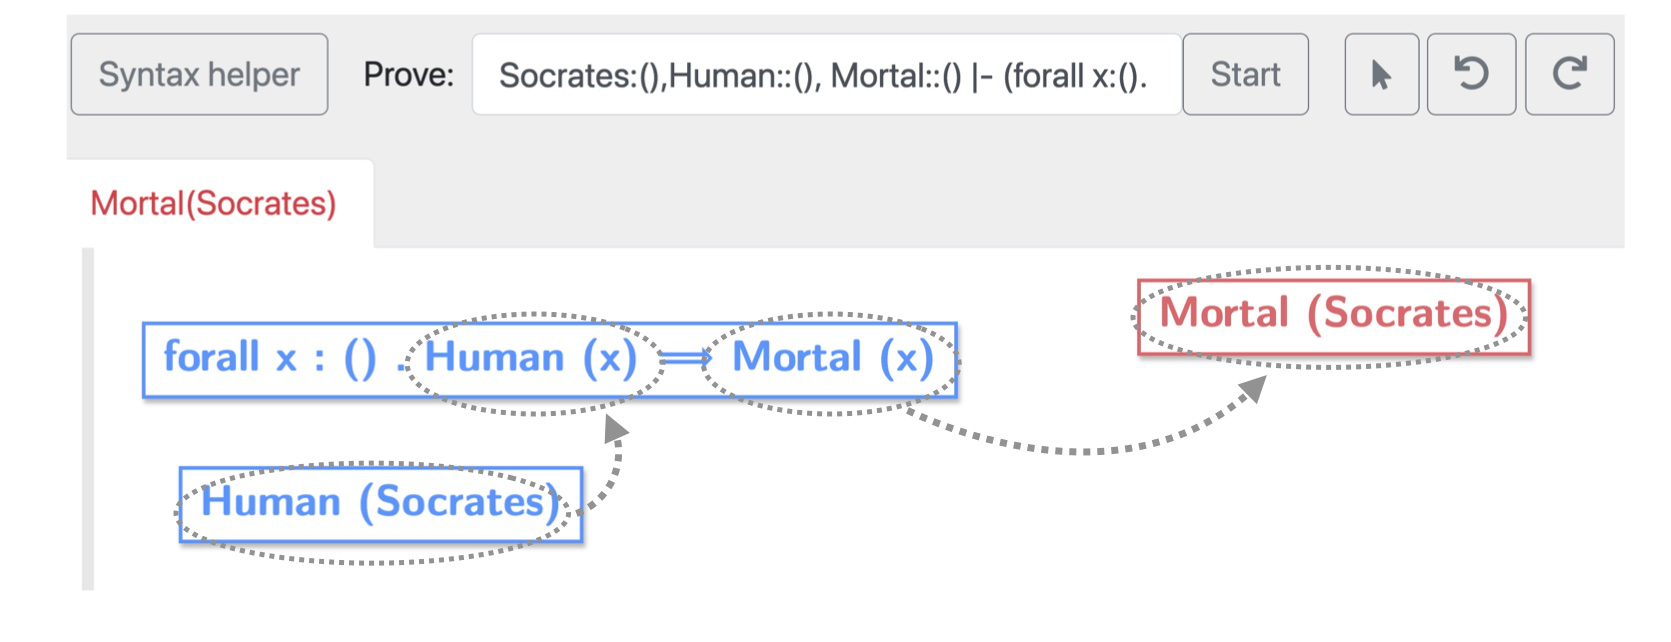
\includegraphics[width=1.3\textwidth]{actions-tag.png}}
 \end{center}
 The conclusion is red on the right, the two hypotheses blue on the left. The
 gray dotted arrows have been added to show the two possible actions.
 \caption{A partial screenshot showing a goal in the Actema prototype}
 \labfig{aristote}
 \end{figure*}

We will not consider, on paper, the details of variable renaming in
substitutions, implicitly applying the so-called Barendregt
convention, that bound and free variables are distinct and that a
variable is bound at most once.

Extending this work to simple extensions of \kl{FOL}, like multi-sorted predicate
calculus is straightforward (and actually done in the Actema prototype). Some
interesting points may show up when considering how to apply this work to more
complex formalisms like type theories. We will not explore these questions here.

% Another interesting question is how our approach extends to classical logic(s),
% by using multi-conclusion sequents. In this chapter we only give a few hints on
% this topic. A more thorough investigation will be done in
% \refsec{sfl-classical}.

\section{A first example}\labsec{aristote}

\subsection{Layout}
One advantage of the PbA paradigm, is that it allows a very lean visual layout
of the proof state. There is no need to name hypotheses. In the prototype we
also dispense with a text buffer, since proofs are solely built through
graphical actions.


\reffig{aristote} shows the layout of the system using the
ancient example from Aristotle. A goal appears as a set of {\em items}
whose nature is defined by their respective colors\sidenote{We are
  well aware that, in later implementations, this color-based
  distinction ought to be complemented by some other visual
  distinction, at least for users with impaired color vision. But in
  the present description we stick to the red/blue denomination, as it
  is conveniently concise.}:
\begin{itemize}
\item A {\em red item} which is the proposition to be proved, that is the
 {\em conclusion},
\item {\em blue items}, which are the local {\em hypotheses}.
\end{itemize}

The items are what the user can act upon: either by {\em clicking} on them, or
by {\em moving} them. Each item can be positioned freely on a so-called
\emph{proof canvas}, which is depicted by the white background in
\reffig{aristote}.

Finally, note that each goal is displayed on a tab.

\subsection{Two kinds of actions}
In this example, there are two possible actions.

\begin{itemize}
\item A first one is to bring together, by drag-and-drop, the red conclusion
$\mortal(\socrates)$ with the succedant of the first hypothesis $\mortal(x)$.
This will transform the goal by changing the conclusion to $\human(\socrates)$.
\item A second possibility is to combine the two hypotheses; more precisely to
bring together the item $\human(\socrates)$ with the premise $\human(x)$ of the
first hypothesis. This will yield a new hypothesis $\mortal(\socrates)$.
\end{itemize}

The first case is what we call a {\em backward step} where the conclusion is
modified by using a hypothesis. The second case is a {\em forward step} where
two known facts are combined to deduce a new fact, that is an additional blue
item.

In both cases, the proof can then be finished invoking the logical
axiom rule. In practice this means bringing together the blue
hypothesis $\human(\socrates)$ (resp. the new blue fact
$\mortal(\socrates)$) with the identical red conclusion.


\subsection{Modelling the mechanism}

A backward step involves a hypothesis, here $\forall x.\-\human(x)
\allowbreak\limp \mortal(x)$ and the conclusion, here $\mortal(\socrates)$.
Furthermore, the action actually links together two {\em subterms} of each of
these items; this is written by squaring these subterms. The symbol ${\back}$,
used as an operator, is meant to describe the result of the interaction.
Internally, the behavior of this operator is defined by a set of rewrite rules
given in \reffig{DISL} and \reffig{DISL-U}. Here is the sequence of
rewrites corresponding to the example\sidenote{Note that $\back$ has lower
precedence than all logical connectives.}: \renewcommand{\arraystretch}{1.1}
$$\begin{array}{lll}
    &  \forall x.\human(x)\limp \select{\mortal(x)} \back \select{\mortal(\socrates)}&\\
    \step{} &
           \human(\socrates)\limp \select{\mortal(\socrates)}
           \back \select{\mortal(\socrates)}&
                                               \mathsf{L\forall i}\\
    \step{} &
           \human(\socrates)\land(\select{\mortal(\socrates)}
           \back \select{\mortal(\socrates)}) &
                                                 \mathsf{L{\limp}_2}\\
    \step{} &  \human(\socrates)\land \top &
                                           \mathsf{id}\\
    \step{} & \human(\socrates)&\mathsf{neur}\\
  \end{array}$$

Notice that:
\begin{itemize}
\item   These elementary rewrites are not visible for the user. What she sees is
  the final result of the action, that is the last expression of the rewrite
  sequence.
\item The definitions of the rewrite rules in \reffig{DISL} and
  \reffig{DISL-U} do not involve squared subterms. The information of which
  subterms are squared is only used by the system to decide which rules to
  apply in which order.
\end{itemize}

In general, the action solves the goal when the interaction ends with
the trivially true proposition $\top$. The base case being the action
corresponding to the axiom/identity rule \rsf{id}: $A\back A \step{} \top$.

A forward step, on the other hand, involves two (subterms of two)
hypotheses. The interaction operator between two hypotheses is written
$\forw$. In the example above, the detail of the interaction is:
$$
  \begin{array}{lll}
    &  \forall x .\select{\human(x)}\limp\mortal(x) \forw \select{\human(\socrates)}&\\
    \step{} & \select{\human(\socrates)}\limp\mortal(\socrates) \forw \select{\human(\socrates)}& \mathsf{F \forall i}\\
    \step{} & (\select{\human(\socrates)}\back \select{\human(\socrates)} )\limp\mortal(\socrates) &\mathsf{F{\limp}_1}\\
    \step{} & \top \limp\mortal(\socrates) &\mathsf{id}\\
    \step{} & \mortal(\socrates) & \mathsf{neul}\\
  \end{array}
$$

The final result is the new hypothesis. We come back to the study of the rewrite
rules of ${\back}$ and ${\forw}$ in \refch{sfl}.


\section{Proof steps through clicks}\labsec{clicks}
Drag-and-drop actions involve two items. Some proof steps involve only
one item; they can be associated to the action of clicking on this
item. The general scheme is that clicking on a connective or quantifier
allows to ``break'' or destruct this connective. The results of clicks
are not very surprising, but this feature is necessary to complement
drag-and-drop actions.
\begin{itemize}
\item Clicking on a blue conjunction $A\land B$ transforms the
    item into two separate blue items $A$ and $B$.
\item Clicking on a red conjunction $A\land B$ splits the goal into
    two subgoals, whose conclusions are respectively $A$ and $B$.
\item Clicking on a blue disjunction $A\lor B$ splits the goal into two subgoals
    of same conclusion, with $A$ (resp. $B$) added as a new hypothesis.
\item Clicking on the left (resp. right)-hand subterm of a red
      disjunction $A\lor B$ replaces this red conclusion by $A$
      (resp. $B$).
\item Clicking on a red implication $A\limp B$ breaks it into a
      new red conclusion $B$ and a new blue hypothesis $A$.
\item Clicking on a red universal quantifier $\forall x.A$ introduces
  a new object $x$ and the conclusion becomes $A$.
\item Clicking on a blue existential $\exists x.A$ introduces a new
  object $x$ together with a blue hypothesis $A$.
\item Clicking on a red equality $t = t$ solves the goal immediately.
\end{itemize}

One can see that these actions correspond essentially to the (right)
introduction rules of the head connective for the conclusion, and either the
elimination rule from \kl{NJ} or the left introduction rule from \sys{LJ} for
hypotheses. The exact mapping between click actions and inference rules is
given in \reftab{click-rules}. A few remarks are in order:
\begin{itemize}
  \item In the current implementation of Actema, clicking on a blue item $A
  \limp B$ will work only if the conclusion is $B$. An alternative is to use the
  {\rsf{{\limp}L}} rule from \kl{sequent calculus}, which is applicable in every
  context.
  \item There is no action mapped to red $\bot$ items, simply because $\bot$
  does not have any introduction rule.
  \item There is currently no action mapped to blue $∀$ and red $∃$ items. The
  reason is that one needs additional information about the \emph{witness} to be
  used when instantiating with the $∀L$ or $∃R$ rule. This could be provided
  with further input (e.g. from a dialog box), but this would need a change in
  the communication protocol between the frontend and backend of Actema. Instead
  we decompose this in two steps: first the user can add the witness as a new
  object by using the \texttt{+expr} button (see \refsec{newitems}); then she
  can drag the corresponding green item and drop it on the quantified item to
  instantiate it. It is also possible to select with the mouse an arbitrary
  subexpression occurring in any item of the current goal, and then
  drag-and-drop the item holding the selected subexpression instead.
\end{itemize}

\begin{remark}[Click completeness]\label{rem:click-completeness}
  From the previous remarks and the completeness of the cut-free sequent
  calculus \kl{LJ}, it follows that click actions, when combined with new
  object declarations and DnD instantiations, provide a sufficient set of
  interactions to prove any true formula of (\kl{intuitionistic}) \kl{first-order logic}.
\end{remark}

\begin{table}[H]
\caption[]{Mapping of click actions to inference rules}
\labtab{click-rules}
\begin{tabular}{ccc}
	\toprule
	\thead{Head connective} & \thead{Red item} & \thead{Blue item} \\
	\midrule
  $\top$ & \rsf{\top R} & \rsf{\top L} \\
	\midrule
  $\bot$ & $\emptyset$ & \rsf{\bot L} \\
	\midrule
	$\land$ & \rsf{\land R} & \rsf{\land L} \\
	\midrule
	$\lor$ & \rsf{\lor R_1, \lor R_2} & \rsf{\lor L} \\
	\midrule
  $\limp$ & \rsf{{\limp}R} & \rsf{{\limp}E} \\
	\midrule
  $∀$ & \rsf{∀R} & $\emptyset$ \\
	\midrule
  $∃$ & $\emptyset$ & \rsf{∃L} \\
\end{tabular}
\end{table}


It is possible to associate some more complex effects to click actions performed
on locations deeper under connectives. This is the essence of Proof-by-Pointing,
and~\sidecite{PbP} provides ample description. Since we here focus more on
drag-and-drop actions, we do not detail further more advanced PbP features.
However we stress that these features are essentially compatible with what we
describe in this work. In fact the version of Actema presented in \refch{plugin}
provides an implementation of PbP available as a contextual menu action.


\section{Adding new items}\labsec{newitems}

Often in the course of a proof, one will want to add new items: either a new
conjecture (blue item), or a new object (green item) that would be helpful to
solve the current goal. These can be done respectively with the blue
\texttt{+hyp} and the green \texttt{+expr} buttons, which appear in the
screenshot of \reffig{edukera}. When clicked, they prompt the user
for the statement of the conjecture, or the name and expression defining the
object. The \texttt{+hyp} button will also create a new subgoal requiring to
prove the conjecture within the current context.

% This mechanism and the syntax are for now very crude. The design of
% possible smoother tools is an important issue but left for future
% work\sidenote{For instance~\cite{omar-filling-2021} deals with a
%   similar problem in the context of functional programming.}.

For now we ask the user to input textual data, in an idiosyncratic syntax
specific to the logic of Actema. A desirable, but highly non-trivial feature
would be to provide some elaborate input mechanism tailored to the type of
object the user wants to create. This would obviously require some extensibility
to new domain-specific input interfaces: typically one could imagine plugging a
tool like GeoGebra to construct geometrical figures \sidecite{gg2}, or a
categorical diagram editor like YADE\todo{add citation/link to Ambroise Lafont's
work}.

% We will not explore the design of such features in this thesis, since we focus
% on finding a universal interface for logical reasoning rather than
% domain-specific interfaces for particular types of mathematical reasoning.  Note
% however that it is a necessary feature if one wants to achieve a fully graphical
% theorem proving environment which is accessible to non-expert users.

\section{A simple example involving equality}\labsec{equality}

Most \kl{interactive theorem provers} expose a \emph{rewrite} tactic that allows the
use of equality hypotheses, that is known equations of the form $t = u$, in
order to replace some occurrences of $t$ by $u$ (or symmetrically, occurrences
of $u$ by $t$). This substitution can be performed in the conclusion or in
hypotheses. Specifying the occurrences to be replaced with textual commands can
be quite tedious, since it involves either dealing with some form of
naming/numbering to designate locations of subterms, or writing manually
patterns which duplicate parts of the structure of terms.

\begin{figure*}
  \begin{center}
    \fbox{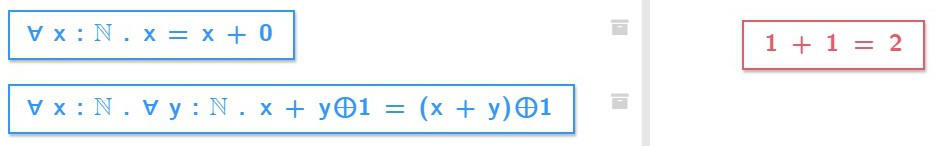
\includegraphics[width=1.3\textwidth]{oneplusone.png}}
  \end{center}
  \caption{Proving $1 + 1 = 2$ in Peano arithmetic}
  \labfig{oneplusone}
\end{figure*}

In our setting we can provide this replacement operation through
drag-and-drop. The user points at the occurrence(s) of $t$ to be
replaced, and then brings them to the corresponding side of the
equality.

\reffig{oneplusone} shows a very elementary example where one wants to prove
$1+1=2$ in the setting of Peano arithmetic. For any number $n$, we write
$\suc{n}$ to denote the application of the successor function to $n$; closed
terms are directly written in decimal notation. The proof goes as follows:
\begin{itemize}
  \item We link the left-hand side $x + \suc{y}$ of the second addition axiom with $1 + 1$ in the conclusion, which has the effect of rewriting $1 + 1$ into $\suc{(1 + 0)}$:
    $$
      \begin{array}{lll}
        & \forall x. \forall y. \select{x + \suc{y}} = \suc{(x + y)} \back \select{1 + 1} = 2 & \\
        \step{} & \forall y. \select{1 + \suc{y}} = \suc{(1 + y)} \back \select{1 + 1} = 2 &\mathsf{L\forall i} \\
        \step{} & \select{1 + \suc{0}} = \suc{(1 + 0)} \back \select{1 + 1} = 2 &\mathsf{L\forall i} \\
        \syneq & \select{1 + 1} = \suc{(1 + 0)} \back \select{1 + 1} = 2 & \\
        \step{} & \suc{(1 + 0)} = 2 &\mathsf{L{=}_1}
      \end{array}
    $$
  \item We link the right-hand side $x + 0$ of the first addition axiom with $1 + 0$ in the conclusion, which rewrites $1 + 0$ into $1$:
    $$
      \begin{array}{lll}
        & \forall x. x = \select{x + 0} \back \suc{(\select{1 + 0})} = 2 & \\
        \step{} & 1 = \select{1 + 0} \back \suc{(\select{1 + 0})} = 2 &\mathsf{L\forall i} \\
        \step{} & \suc{1} = 2 &\mathsf{L{=}_2} \\
        \syneq & 2 = 2 &
      \end{array}
    $$
\end{itemize}

We end up with the conclusion $2 = 2$, which is provable by a simple click.
Notice how the orientation of the two rewritings is determined by which side of
the equality is selected. Also, in this case, the rewritings
correspond to backward proof steps, because the rewriting is performed
in the conclusion. Similar rules (\rsf{F{=}_1} and \rsf{F{=}_2}) are
used to perform rewritings in hypotheses.


\section{Drag-and-dropping through connectives}\labsec{dnd-examples}
We mentioned in \refsec{clicks} that it is possible to destruct logical
connectives through click actions. In many cases however, this will not be
necessary: because a drag-and-drop involves subterms of the items involved, one
can often directly use (resp. act on) the part of the hypothesis (resp.
conclusion) which is of interest.

\subsection{Conjunction and disjunction}
The conjunction is an easy to explain case. A hypothesis of the form
$A\land B$ can be used directly both as evidence for $A$ and as evidence
for $B$. This is modeled by the rules \rsf{L\land_1} and
\rsf{L\land_2}. A very simple action is thus:
$$
\begin{array}{llll}
  \select{A}\land B \back \select{A} & \step{}& \select{A} \back
  \select{A} \hbox to 1cm {\hfil}&\mathsf{L \land_1}\\
                                       & \step{} &\top & \mathsf{id}
\end{array}
$$

On the other hand, considering a conjunctive goal $A\land B$, one can
simplify or solve one of the branches by a DnD action. This involves
rules \rsf{R \land_1} and
\rsf{R \land_2}. For instance:
$$
\begin{array}{llll}
  \select{A} \back \select{A}\land B &
                                         \step{}& (\select{A} \back
                                         \select{A})\land B &\mathsf{R \land_1}\\
                                       & \step{}& \top \land B  & \mathsf{id}\\
  &\step{}& B&\mathsf{neul}
\end{array}
$$

Red disjunctions work similarly to conjunctive goals, except that solving one
branch will solve the entire goal. A nice consequence of this, which is hard to
simulate with textual tactics, is that one can just simplify one branch of a
disjunction without comitting to proving it entirely:
$$
\begin{array}{llll}
  \select{A} \back (B \land \select{A}) \lor C
    & \step{} & (\select{A} \back B \land \select{A}) \lor C &\mathsf{R\lor_1}\\
    & \step{} & (B \land (\select{A} \back \select{A})) \lor C &\mathsf{R\land_2}\\
    & \step{} & (B \land \top) \lor C &\mathsf{id}\\
    & \step{} & B \lor C &\mathsf{neur}
\end{array}
$$

Disjunctive hypotheses also have a backward behavior defined by the rules
\rsf{L\lor_1} and \rsf{L\lor_2}, although in most cases one will prefer the
usual subgoal semantics associated with click actions. More interesting is
their forward behavior with the rules \rsf{F\lor_1} and \rsf{F\lor_2}, in
particular when they interact with negated hypotheses. For instance:
$$
\begin{array}{llll}
  \select{A} \lor B \forw \neg \select{A}
    & \step{} & (\select{A} \forw \neg\select{A}) \lor B &\mathsf{F\lor_1}\\
    & \step{} & \neg (\select{A} \back \select{A}) \lor B &\mathsf{F{\limp}_1}\\
    & \step{} & \neg \top \lor B &\mathsf{id}\\
    & \step{} & \bot \lor B &\mathsf{neul}\\
    & \step{} & B &\mathsf{neul}\\
\end{array}
$$

We have noticed that on some examples, such actions could provide a
significant speed-up with respect to traditional textual command
provers. We give a more concrete example in \refsec{edukera}.

Notice that we used rules associated with implication, since negation can be
defined by $\neg A \defeq A \limp \bot$.

\subsection{Implication}\labsec{implication}
The implication connective is crucial, because it is not monotone. More
precisely, the roles of hypotheses and conclusions are reversed on the
left of an implication. We start with some very basic examples
for the various elementary cases.

Using the right hand part of a hypothesis $A\limp B$ turns a 
conclusion $B$ into $A$. 
$$
\begin{array}{llll}
  A\limp \select{B} \back \select{B} &\step{}& A\land (\select{B}
                                                \back
                                                \select{B})&\mathsf{L
                                                             {\limp}_2}\\
                                         &\step{}&A\land\top & \mathsf{id}\\
    &\step{}& A&\mathsf{neul}
\end{array}
$$

This can also be done under conjunctions and/or disjunctions:
$$
  A\limp \select{B} \back C \land (D\lor \select{B}) ~~ \steps{} ~~ C \land (D\lor A)
$$

An interesting point is what happens when using implications with
several premisses. The curried and uncurried versions of the
implication will behave exactly the same way:

$$
  A\limp B \limp \select{C} \back D\lor \select{C}
  ~~~\/ ~\steps{}~~~  D\lor (A\land B)
$$
and:
$$
  A\land B \limp \select{C} \back D\lor \select{C}
  ~~~ \/ ~\steps{}~~~  D\lor (A\land B)
$$


As we have seen in Aristotle's example (\refsec{aristote}), blue
implications can also be used in forward steps, where another
hypothesis matches one of their premisses.

A first nice feature is the ability to strengthen a hypothesis by
providing evidence for any of its premises:
$$
B\limp \select{A}\limp C \forw \select {A}  ~~\/~\/~\steps{}~\/~~~~~
B\limp C$$
and again the same can be done for the uncurryfied version:
$$
B\land \select{A}\limp C \forw \select {A}  ~\/~\/~\steps{}~\/~~~~~
B\limp C.$$

The two aspects of the implication can be combined:

$$
B\limp \select{A}\limp C \forw D\limp\select {A}  ~\/~\/~\steps{}~\/~~~~~
B\limp D\limp C$$
or:
$$
B\land \select{A}\limp C \forw D\limp\select {A}  ~\/~\/~\steps{}~\/~~~~~
B\land D \limp C.$$


Note that there is almost no difference in the way one uses different
versions of a hypothesis $A\limp B\limp C$, $A\land B\limp
C$, but also $B\limp A\limp C$, in forward as well as in
backward steps\sidenote{When viewed as types through the Curry-Howard
isomorphism, $A\limp B\limp C$, $A\land B\limp C$, $B\land
A\limp C$ and $B\limp A\limp C$ are {\em isomorphic types};
and Roberto di Cosmo~\cite{ISOSBook} has also precisely underlined
that type isomorphisms should help to free the programmer from
arbitrary syntactical choices.}. This underlines, we hope, that our
proposal makes the proof construction process much less dependent on
arbitrary syntactical details, like the order of hypotheses or whether
they come in curryfied form or not.

Also, the rules for implication combined with the rules for equality
\rsf{L{=}_i} or \rsf{F{=}_i} naturally give access to {\em
  conditional rewriting}; we detail this in combination with
quantifiers in the next section.

%A powerful property of our rewrite rules is that this behavior is true at
%\emph{any depth} under logical connectives.


As for red implications, they also have a backward semantics with the rules
\rsf{R{\limp}_1} and \rsf{R{\limp}_2}, but most of the time one
will want to destruct them immediately by click. An exception could be if one
wants to simplify some part of an implicative, inductive goal before starting
the induction.

\subsection{Quantifiers}
As the first example of this chapter shows, drag-and-drop actions work through
quantifiers and can trigger instantiations of quantified variables. This is made
possible by the rules \rsf{L\forall i} and \rsf{F\forall i}, which allow the
instantiation of a variable universally quantified in a hypothesis.

Symmetrically, a variable quantified existentially in a conclusion can
also be instantiated. For instance:

$$\begin{array}{llll}
    \select{A(t)}\back \exists x.\select{A(x)}&\step{}&
                                                      \select{A(t)}\back\select{A(t)}&\mathsf{L}\forall\mathsf{i}
    \\
                                               &\step{}& \top&\mathsf{id}
  \end{array}
  $$

An interesting feature is the possibility to modify propositions under
quantifiers. Consider the following possible goal:
% Take this example involving equality:
% $$\begin{array}{clc}
%    & \forall x.\select{ x+0 = x }\back \forall a. \select{a+0} = 0 +
%      a&  \\
%          \step{}&\forall a.(\forall x.\select{x+0 = x }\back \select{a+0} =
%             0 +a)&\mathsf{R}\forall\mathsf{s}\\
%      \step{}&\forall a. (\select{a+0=a}\back  \select{a+0} = 0 +a)& \mathsf{L}\forall\mathsf{i}\\
%      \step{}&\forall a. a = 0+a&\mathsf{L}=1
%                                \end{array}$$
% Performing such a transformation of the goal $\forall a.a+0=0+a$
% without destroying the head quantifier is not trivial traditional
% provers; here it is done through one simple action.
$$\forall a.\exists b. A(f(a)+g(b))$$
where $A$, $f$ and $g$ can be complex expressions. Suppose we have a
lemma allowing us to prove:
$$\forall a.\exists b. A(g(b)+ f(a)).$$
Switching from one formulation to the other, involves one use of the
commutativity property $\forall x.\forall y. x+y=y+x$.
% But because this has to be performed under two quantifiers, doing this in
% traditional interactive theorem provers can be tedious. For instance in Coq, one
% must use a specific tactic called \texttt{setoid_rewrite}.
In our setting, the equality can be used under quantifiers in one single action:
$$
\begin{array}{ll}
  &\forall x.\forall y. \select{x+y}=y+x \back \forall a.\exists b. A(\select{f(a)+g(b)})\\
\steps{} & \forall a.\exists b. A(g(b)+f(a))
\end{array}$$


Note also that it is possible to instantiate only some of the universally
quantified variables in the items involved. In general, a universally
quantified variable can be instantiated when the quantifier is in a
negative position; for instance:
%\setlength{\abovedisplayskip}{-5pt}
%\setlength{\belowdisplayskip}{0pt}
%\setlength{\belowdisplayshortskip}{0pt}
$$
\begin{array}{rcl}
 \forall x.\forall
 y. \select{P(y)}\limp R(x,y)\forw \select{P(a)} ~\/~\steps{}
~\/~ \forall x. R(x,a)
 %% \\
 %% \mbox{\hbox to 0pt{\hss or equivalently:}}
 %% \forall y.\forall
 %% x. \select{P(x)}\limp R(x,y)\forw \select{P(a)} \steps{}
 %% \forall y. R(a,y)
\end{array}
$$
This last example illustrates how partial instantiation abstracts away the order
in which quantifiers are declared, very much like the partial application
presented earlier for implication\sidenote{This fact should not be too
surprising to the reader familiar with dependent type theory, where implication
is usually defined as a special case of universal quantification.}.
%% What the last example stresses is, again, that syntactical details,
%% here the order in which variables are quantified, are much less
%% relevant in the gestual proof constructions than in their textual
%% counterparts.


Again, in some cases, only some existential quantifiers may be
instantiated following a linkage:
$$
\begin{array}{rcl}
\select{P(a)}\back \exists x.\exists y. \select{P(y)}\land R(x,y)
 ~\/~\steps{}
~\/~
    \exists x. R(x,a)
\end{array}
$$

When using an existential assumption, one can either destruct it
through a click, or use or transform it through a DnD; for instance:
$$
\exists x.\select{P(x)}\forw \forall y.\select{P(y)}\limp
Q(y)  ~\/~\steps{}
~\/~\exists x.Q(x)
$$

\subsection{Dependency between variables}\labsec{acyclicity}
Some more advanced examples yield simultaneous instantiations of
existentially and universally quantified variables. In such cases, the
system needs to check some dependency conditions. For instance, the
following linkage is valid and solves the goal through one action:
$$
\begin{array}{lll}
  &\exists y. \forall x. \select{R(x,y)}\back \forall x'.\exists
    y'. \select{R(x',y')}& \\
  \step{}& \forall y.(\forall x. \select{R(x,y)}\back \forall x'.\exists
        y'. \select{R(x',y')} ) \mbox{\hbox to 12pt{\hfill}}& \mathsf{L}\exists\mathsf{s}\\
  \step{} &\forall y. \forall x'. (\forall x. \select{R(x,y)}\back \exists
  y'. \select{R(x',y')} ) ~~~~~~~~~~~~&\mathsf{R}\forall\mathsf{s}\\
  \step{} &  \forall y. \forall x'. (\forall
         x. \select{R(x,y)}\back\select{R(x',y)} )&\mathsf{R}\exists\mathsf{i}\\
  \step{}&   \forall y. \forall
           x'. (\select{R(x',y)}\back\select{R(x',y)} )&\mathsf{L}\forall\mathsf{i}\\
   \step{}  &  \forall y. \forall
           x'. \top & \mathsf{id}\\
\steps{}& \top
\end{array}
$$

But the converse situation is not provable; the system will refuse
the following linkage:
$$
\begin{array}{rcl}
  \forall x. \exists y. \select{R(x,y)}\back \exists y'.\forall x'. \select{R(x',y')}
\end{array}
$$
Indeed, there is no reduction path starting from this linkage ending with the
\textsf{id} rule. This can be detected by the system because the unification of
$R(x,y)$ and $R(x',y')$ here results in a cycle in the instantiations of
variables\sidenote{We will come back to this in \refsec{linkages}. Also notice
that this example requires to use full (first-order) unification, not only
matching.}. The system thus refuses this action.

\subsection{Conditional rewriting}
The example given in \refsec{equality}, although very simple,
already combines the rules for equality and for quantifiers. When also
using implication, one obtains naturally some form of conditional
rewriting. To take another simple example, suppose we have a
hypothesis of the form:
$$\forall x. x\neq 0 \limp f(x) = g(x)$$

We can use this hypothesis for replacing a subterm $f(t)$ by $g(t)$,
which will generate a side-condition $t\neq 0$:
$$
\begin{array}{lll}
  &\forall x. x\neq 0 \limp \select{f(x)} = g(x) \back A(\select{f(t)}) &\\
  \step{} & t\neq 0 \limp \select{f(t)} = g(t) \back A(\select{f(t)}) &\mathsf{L \forall i}\\
  \step{} & t\neq 0 \land (\select{f(t)} = g(t) \back A(\select{f(t)})) & \mathsf{L{\limp}_2}\\
  \step{} &  t\neq 0 \land A(g(t)) &\mathsf{L{=}_1} \\
\end{array}$$

One could similarly do such a rewrite in a hypothesis. Furthermore,
the conditional rewrite can also be performed under quantifiers; for instance:
$$
\begin{array}{lll}
  &\forall x. x\neq 0 \limp \select{f(x)} = g(x) \back \exists y . A(\select{f(y)})
  &\mathsf{R \exists s}\\
  \step{} &\exists y. ( \forall x. x\neq 0 \limp \select{f(x)} = g(x) \back A(\select{f(y)})) &\mathsf{L \forall i}\\
  \step{} & \exists y. ( y\neq 0 \land ( \select{f(y)} = g(y) \back A(\select{f(y)}) )) &\mathsf{L{\limp}_2} \\
  \step{} & \exists y .( y\neq 0 \land A(g(t))) &\mathsf{L{=}_1} \\
\end{array}$$


% \todo{Remove page break (while keeping the wide page layout for the rules).}

\pagelayout{wide} % No margins
\begin{figure}
  \fontsize{10}{10.5}\selectfont
    \renewcommand{\arraystretch}{1.25}
  \begin{framed}
  \begin{mathpar}
    \begin{array}{r@{\quad}c@{\quad}lr}
        \multicolumn{4}{c}{\textsc{Backward}} \\[2em]

        {A \back A}&\step{}&\top &\mathsf{id}\\
        {t = u \back \subst{A}{t}{x}}&\step{}&\subst{A}{u}{x} &\mathsf{L{=}_1}\\
        {t = u \back \subst{A}{u}{x}}&\step{}&\subst{A}{t}{x} &\mathsf{L{=}_2}\\[1em]

        {(B \land C) \back A}&\step{}&        {B \back A}&\mathsf{L \land_1}\\
        {(C \land B) \back A}&\step{}&        {B \back A}&\mathsf{L \land_2}\\
        {A \back~(B \land C)}&\step{}&        {(A \back B) \land C}&\mathsf{R \land_1}\\
        {A \back~(C \land B)}&\step{}&        {C \land (A \back B)}&\mathsf{R \land_2}\\[1em]
        
        {(B \lor C) \back A}&\step{}&        {(B \back A) \land (C \limp A)}&\mathsf{L \lor_1}\rever\\
        {(C \lor B) \back A}&\step{}&        {(C \limp A) \land (B \back A)}&\mathsf{L \lor_2}\rever\\
        {A \back~(B \lor C)}&\step{}&        {(A \back B) \lor C}&\mathsf{R \lor_1}\\
        {A \back~(C \lor B)}&\step{}&        {C \lor (A \back B)}&\mathsf{R \lor_2}\\[1em]

        {(C \limp B) \back A}&\step{}&        {C \land (B \back A)}&\mathsf{L{\limp}_2}\\
        {A \back~(B \limp C)}&\step{}&        {(A \forw B) \limp C}&\mathsf{R{\limp}_1}\rever\\
        {A \back~(C \limp B)}&\step{}&        {C \limp (A \back B)}&\mathsf{R{\limp}_2}\rever\\[1em]

        % {A \back \neg B}&\step{}&        {\neg (A \forw B)}&\mathsf{R\neg}\rever\\[1em]

        {(\forall x. B) \back A}&\step{}&        {\subst{B}{x}{t} \back A}&\mathsf{L \forall i}\\
        {(\forall x. B) \back A}&\step{}&        {\exists x. (B \back A)}&\mathsf{L \forall s}\\
        {A \back~(\forall x. B)}&\step{}&        {\forall x. (A \back B)}&\mathsf{R \forall s}\rever\\[1em]

        {(\exists x. B) \back A}&\step{}&        {\forall x. (B \back A)}&\mathsf{L \exists s}\rever\\
        {A \back~(\exists x. B)}&\step{}&        {A \back \subst{B}{x}{t}}&\mathsf{R \exists i}\\
        {A \back~(\exists x. B)}&\step{}&        {\exists x. (A \back B)}&\mathsf{R \exists s}\\
    \end{array}
  % \end{mathpar}
  \and
  % \textsc{Forward}\\
  % \begin{mathpar}
    \begin{array}{r@{\quad}c@{\quad}lr}
      \multicolumn{4}{c}{\textsc{Forward}} \\[2em]

      % \R[\mathsf{lnn}]
      %   {\ifill{\eta}{\efill{A}{A} \forw \efill{B}{B}}}
      %   {\ifill{\eta}{\ifill{A}{A} \land \ifill{B}{B}}}
      % \\
      {\subst{A}{t}{x} \forw~(t = u)} &\step{}& {\subst{A}{u}{x}}&\mathsf{F{=}_1}\\
      {\subst{A}{u}{x} \forw~(t = u)} &\step{}& {\subst{A}{t}{x}}&\mathsf{F{=}_2}\\[1em]

        {A \forw~(B \land C)} &\step{}&   {A \forw B}&\mathsf{F\land_1}\\
        {A \forw~(C \land B)}&\step{}&        {A \forw B}&
            \mathsf{F \land_2}\\[1em]

        {A \forw~(B \lor C)}& \step{}&       {(A \forw B) \lor C}
      &
      \mathsf{F \lor_1}\\
        {A \forw~(C \lor B)}&\step{}&        {C \lor (A \forw B)}&
            \mathsf{F \lor_2}\\[1em]

        {A \forw~(B \limp C)}
&\step{}&        {(A \back B) \limp C}
      &\mathsf{F{\limp}_1}\\
        {A \forw~(C \limp B)}&\step{}&        {C \limp (A \forw B)}&
            \mathsf{F{\limp}_2}\\[1em]

%         {A \forw \neg B}
% &\step{}&        {\neg (A \back B)}
%       &\mathsf{F\neg}\\[1em]

        {A \forw~(\forall x. B)}
&\step{}&        {A \forw \subst{B}{x}{t}}
      &
      \mathsf{F \forall i}\\
        {A \forw~(\forall x. B)}&\step{}&        {\forall x. (A \forw B)}&
            \mathsf{F \forall s}\\[1em]

              {A \forw~(\exists x. B)}&\step{}&{\exists x. (A \forw B)}&
              \mathsf{F \exists s}\rever\\[1em]
              
          {B \forw A}&\step{}&
          {A \forw B}& \mathsf{Fcomm}\\
    \end{array}
    \end{mathpar}
    ~\\[1em]
    In the rules $\{\mathsf{L \forall s}, \mathsf{L \exists s}, \mathsf{R \forall
    s}, \mathsf{R \exists s}, \mathsf{F \forall s}, \mathsf{F \exists s}\}$, $x$
    is not free in $A$.
  \end{framed}
  \caption{Linking rules}
  \labfig{DISL}
\end{figure}

\begin{figure}
  \fontsize{10}{10.5}\selectfont
  \begin{framed}
  {\textsc{Units}}\\
  \begin{mathpar}
    \renewcommand{\arraystretch}{1.2}
    \begin{array}{lr@{\quad}c@{\quad}lc}
   \pair{\mcirc}{\dagger} \in \{
      \pair{\land}{\top},
      \pair{\lor}{\bot},
      \pair{\limp}{\top}
      \}&
      {\dagger \mcirc A}&\step{}&A&\mathsf{neul}\\
 \pair{\mcirc}{\dagger} \in \{
      \pair{\land}{\top},
      \pair{\lor}{\bot}
      \}&
      {A \mcirc \dagger}&\step{}&A&\mathsf{neur}\\
   \pair{\mcirc}{\dagger} \in \{
      \pair{\land}{\bot},
      \pair{\lor}{\top}
      \}&
      {\dagger \mcirc A}&\step{}&\dagger&
       \mathsf{absl}\\
  \pair{\mcirc}{\dagger} \in \{
      \pair{\land}{\bot},
      \pair{\lor}{\top},
      \pair{\limp}{\top}
      \}&
      {A \mcirc \dagger}
      &\step{}&\dagger& \mathsf{absr}\\
  \pair{\mdiam}{\dagger} \in \{
    \pair{\forall}{\top},
    \pair{\exists}{\bot}
    \}&      {\mdiam x. \dagger}&\step{}&\dagger&    \mathsf{absq}
    \\
&      {\bot \limp A}&\step{}&\top&\mathsf{efq} 
      \end{array}
  \end{mathpar}
  \end{framed}
  % \begin{framed}
  % {\sc Resources}
  % \begin{mathpar}
  %   %\R[\mathsf{conp}]
  %   %  {\pi\{A \lor A\}}
  %   %  {\pi\{A\}}
  %   %\and
  %   \R[\mathsf{conn}]
  %     {\ifill{\eta}{A \land A}}
  %     {\ifill{\eta}{A}}
  %   \and
  %   \R[\mathsf{wkn}]
  %     {\ifill{\eta}{\top}}
  %     {\ifill{\eta}{A}}
  % \end{mathpar}
  % \end{framed}
  \caption{Unit elimination rules}
  \labfig{DISL-U}
\end{figure}
\pagelayout{margin} % Restore margins

\section{Related works}\labsec{pba-rw}

\paragraph{Window inference}

We have already mentioned Proof-by-Pointing, which was part of the CtCoq and
Pcoq efforts \sidecite{amerkad-mathematics-2001} to design a graphical user
interface for the Coq proof assistant. Another contemporary line of work was the
one based on \emph{window inference}, also mentioned in \refsec{intro-rw}. In
\sidecite{robinson-formalizing-1993}, window inference is described as a general
proof-theoretical framework, which aims to accomodate for the pervasive use of
\emph{equivalence transformations} throughout mathematics and computer science.

% In \cite{robinson-formalizing-1993}, they describe it as a new kind
% of proof-theoretic framework, which aims to accomodate for the pervasive use of
% \emph{equivalence transformations} throughout mathematics and computer science.
% For this purpose, it provides facilities for describing how to focus on specific
% subexpressions, and perform transformations on them that preserve a given
% equivalence relation, while keeping and exploiting information from the context
% where they occur. It is noted in \cite{grundy-window-1991} that the framework
% can be extended to more general relations like preorders, which might typically
% be used to capture the entailment relation of a logic.
Window inference has been used both for general-purpose logics like HOL
\sidecite{grundy-window-1991}, and in more specialized settings like program
refinement \sidecite{grundy-window-1992}. It naturally lends itself to
integration in a graphical user interface
\sidecite{langbacka-tkwinhol-1995,goos-tas-2000}, where the user can
\emph{focus} on a subexpression by clicking on it. One is then presented with a
new \emph{graphical} window, holding the selected expression as well as an
extended set of hypotheses exposing information inferrable from the context of
the expression. The user can pick from a list of valid transformations to be
applied to the expression, before closing the window. This propagates the
transformations to the parent window by replacing the old subexpression by the
new one, without modifying the surrounding context.

This process is quite reminiscent of the rewriting produced by our DnD
actions. One key difference is that window inference rules can be
applied stepwise, while we choose to hide the sequence of rules that
justifies a DnD. The window inference approach gives to the user a
precise control of the transformations to be performed and thus could
inspire interesting extensions of our work.

% This is because
% DnD actions embody the specific intent of justifying an \emph{expression} by
% another \emph{user-specified} expression, which is either assumed to be, or
% trivially equivalent. In contrast, window inference is about justifying the
% \emph{equivalence} of an expression to another, \emph{not yet specified}
% expression. Another way to see it is that our ``link inference'' technique aims
% to capture the process of \emph{applying} some knowledge, while window inference
% provides an interface for the \emph{construction} of new knowledge. They thus
% appear as equally valid and even complementary approaches, that could benefit
% from being implemented in the same interface.


\paragraph{Other gestural proof systems}

There are other proof systems which include drag-and-drop features. Two of them
are the KeY Prover \sidecite{ahrendt-using-2016} and TAS
\sidecite{goos-tas-2000}. TAS is a window inference system tailored for program
refinement, and uses DnD actions between an expression and a transformation, in
order to apply the latter to the former.
%This is obviously different from our use of DnD between entities
%of the same kind, and can be explained by the comparison made in the previous
%paragraph.
As for the KeY Prover, its usage of DnD overlaps only a very small
portion of usecases that we hinted at in \refsec{edukera}, namely
the instantiation of quantifiers with objects.

We can also mention the recent work of Zhan et al. \sidecite{zhan-design-2019}.
They share with us the vision of a proof assistant mainly driven by gestural
actions, which requires far less textual inputs from the user. However, they
only consider point-and-click actions, and rely on a text-heavy presentation at
two levels:
\begin{enumerate}
  \item the proof state, which is a structured proof text in the style of
  Isar~\sidecite{isar};
  \item the proof commands, which can only be performed through choices in
  textual menus.
\end{enumerate}

% The latter can be useful to integrate specific actions which do not fit
% naturally in the gestural paradigm. But because basic reasoning with logical
% connectives and equations occurs so often in virtually any proof, we believe it
% deserves a special treatment in the interface, and our work shows that
% drag-and-drop gestures can be used efficiently for that purpose. This was
% already a concern in \cite{amerkad-mathematics-2001}, where PbP is seen as a
% mean to \emph{``increase the bandwidth between the user and the logical
% engine''}, along with other devices like advanced graphical notations. The
% authors also described how PbP is partially compatible with the production
% \emph{in real time} of a proof text in quasi-natural language, thus close to an
% Isar proof. We conjecture that our drag-and-drop mechanism also has this
% capability, and in fact solves some of the problems induced by the limitation of
% PbP to a single selection.


\paragraph{Explicit proof objects}

Finally let us mention various recent implementations proposing various ways to
construct proofs graphically: Building Blocks~\sidecite{buildingblocks}, the
Incredible Proof Machine~\sidecite{blanchette-visual-2016},
Logitext\sidenote{\url{http://logitext.mit.edu/main}} and Click \&
coLLecT~\sidecite{clickcollect}. In particular, Logitext and Click \& coLLecT
exploit the same idea of associating click actions on head connectives to
inference rules in \kl{sequent calculus}. But these systems focus more on explicating
the proof object than on making its construction easier.